\section{SDK v2- azure-ai-ml}
\subsection{Introduction}
% Style: caption={See comment},captionpos=b]
\paragraph{Difference}
The \gls{g_Python} \gls{AMLSDKv2} with the package library
\begin{center}
	\textbf{azure-ai-ml}
\end{center}
and the \gls{AMLSDKv1} with 
\begin{center}
	\textbf{azureml-core}
\end{center}
are \gls{API}s for the \gls{AML} workspace and it's services. The \gls{CLI} package for \gls{AML} contains a more compact command line style workflows, that need to be executed. The format in v2 is normally \textit{<noun><verb><option>}.\\

The \gls{SDK} is more directed to the development, while the \gls{CLI} is more convient for a \gls{CI}/\gls{CD} process. The later is due to the more compact way of executing commands.\footnote{Reference: \href{https://learn.microsoft.com/en-us/answers/questions/1395777/what-is-the-difference-between-azure-ail-ml-and-az}{Difference CLI, SDK}, \href{https://github.com/microsoft/MLOps}{MLOps Python AML}
}

\paragraph{Azureml-Example: Jobs/single-steps}
For \gls{AML} are provided many examples, that explain the whole process from developing to the full \gls{MLOps} cycle.
For this section, the focus will be on replicating one specific example for the library \textit{scikit-learn} for the dataset \textit{diabetes}. The example can be found under:\\ 
\verb+azureml-examples-main/skd/python/jobs/single-step/scikit-learn/diabetes+.

\begin{figure}[H]
	\centering
	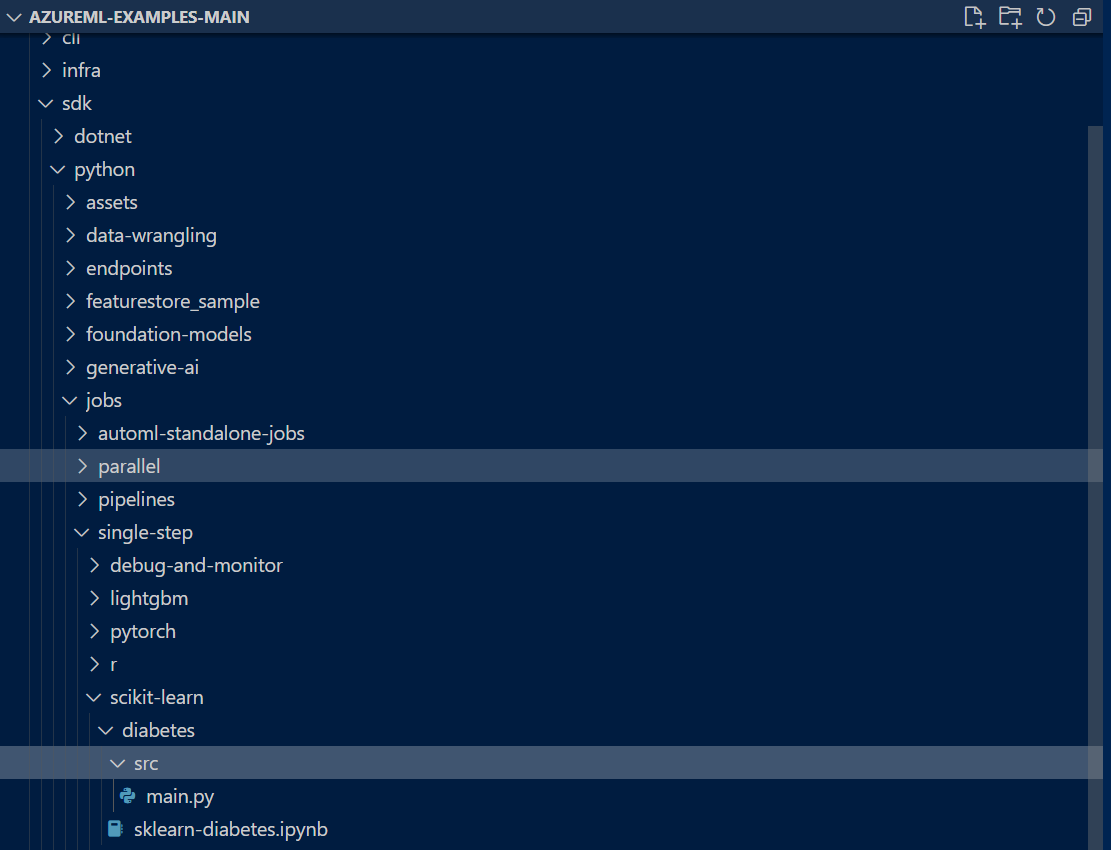
\includegraphics[scale = 0.4]{attachment/chapter_AML/Scc028}
	\caption{One specific example in repo azureml-examples-main}
\end{figure}
Note, that the other repos are present under \verb+GitHub_Notizen_DSci\scripts+ with \gls{AML} in mind:
\begin{itemize}
	\item MLOpsPython-master
	\item mlops-template-for-Azureml-sdk-v2-main,
\end{itemize}
are given a guided tour, how to setup the \gls{MLOps} process. Under \verb+...\scripts\azureml-examples-main+ are also information presented, how to setup the \gls{MLOps}.

\paragraph{Azureml-Example: featurestore samples/sdk only*}
At the moment it is unclear, what the difference is between the previous section and this one. However under\\
\verb+azureml-examples-main/skd/python/featurestore_sample/notebooks/sdk_only/2. Experiemtn and train models using features.ipynb+. is also a approach.


Further documentation can be found here:
\begin{itemize}
	\item \href{https://learn.microsoft.com/de-de/azure/machine-learning/how-to-setup-vs-code?view=azureml-api-2}{Start Setup VS-Code}
	\item \href{https://learn.microsoft.com/de-de/azure/machine-learning/how-to-launch-vs-code-remote?view=azureml-api-2&tabs=vscode-desktop}{Case: VSCode Desktop}
	\item \href{https://learn.microsoft.com/de-de/azure/machine-learning/tutorial-train-deploy-image-classification-model-vscode?view=azureml-api-2}{Tutorial: Reference SDK/CLI v2 Example Doc}
	\item \href{https://github.com/Azure/azureml-examples/blob/main/cli/jobs/single-step/tensorflow/mnist/src/train.py}{azureml-examples/ Tensorflow}
\end{itemize}



\subsection{Connecting to the Workspace}
\subsubsection{Jupyter Notebook using the ikernel from Compute Instance}
Reference: \href{https://learn.microsoft.com/de-de/azure/machine-learning/how-to-launch-vs-code-remote?view=azureml-api-2&tabs=vscode-desktop}{Getting started with VS-Code Desktop}\\

With this functionality, any local \gls{g_JupyterNotebook} can use the a remote server connection to execute code on a compute instance with a \gls{g_Kernel_Jy}.\\

To run a \gls{g_JupyterNotebook}, a \gls{g_Kernel_Jy} needs to be selected.

\begin{figure}[H]
	\centering
	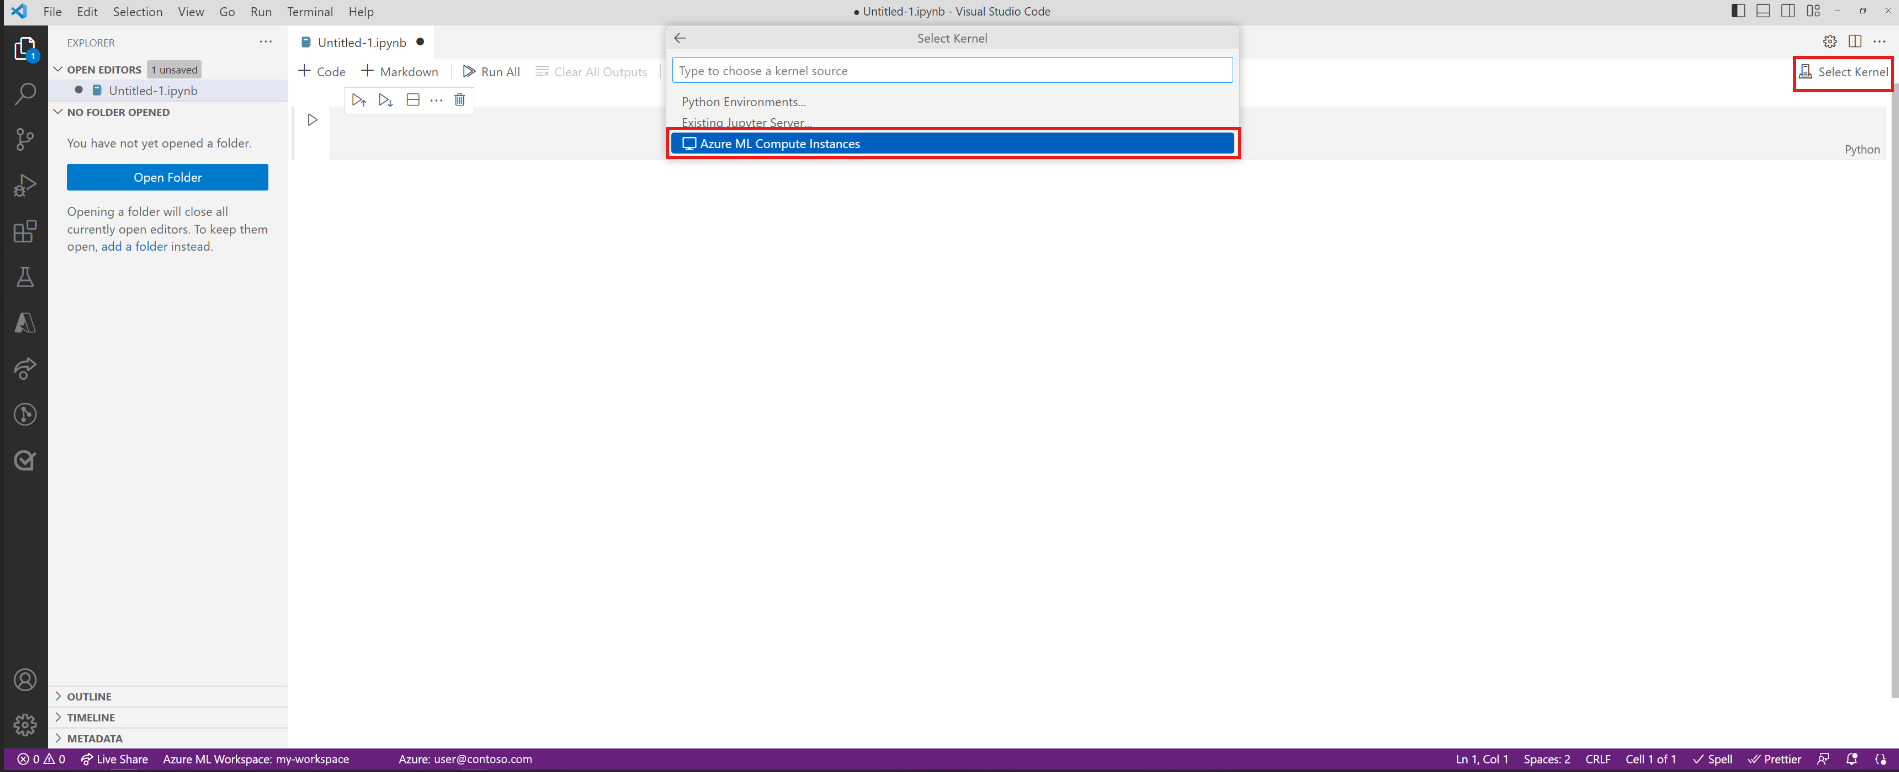
\includegraphics[scale = 0.3]{attachment/chapter_AML/Scc015}
	\caption{Kernel Selection in a Jupyter Notebook}
\end{figure}

In \gls{vsc}, there are multiple options to select a \gls{g_Kernel_Jy}. With the Azure ML extension, the option \textit{Azure ML Compute Instance} is available to.  On the compute instance, a variety of \gls{g_Kernel_Jy} are pre-installed.
\begin{figure}[H]
	\centering
	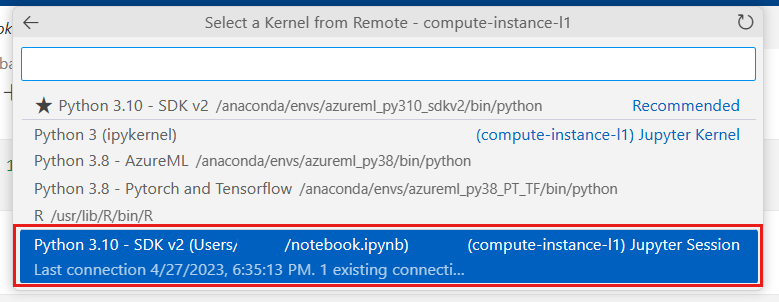
\includegraphics[scale = 0.3]{attachment/chapter_AML/Scc016}
	\caption{Kernel Sources}
\end{figure}

This connection allows to utilize the Azure ML Compute Instance, not all the other resource's. In the following the interaction between and to the other resources will be discussed.

\paragraph{Problem $\&$ Fix: Unable to connect}
One problem accrued. 
\begin{figure}[H]
	\centering
	
\includegraphics[scale = 0.3]{attachment/chapter_AML/Scc017}
	\caption{Error message after selecting Azure ML Compute Instance}
\end{figure}

For the moment, rollback the \gls{g_JupyterNotebook} extension to a version v2023.10.xxx helped.\footnote{
	\href{https://github.com/microsoft/vscode-jupyter/issues/14925}{Posted Problem}, \href{https://github.com/microsoft/vscode-jupyter/pull/14929}{Pull Request and Workaround}
}
\begin{figure}[H]
	\centering
	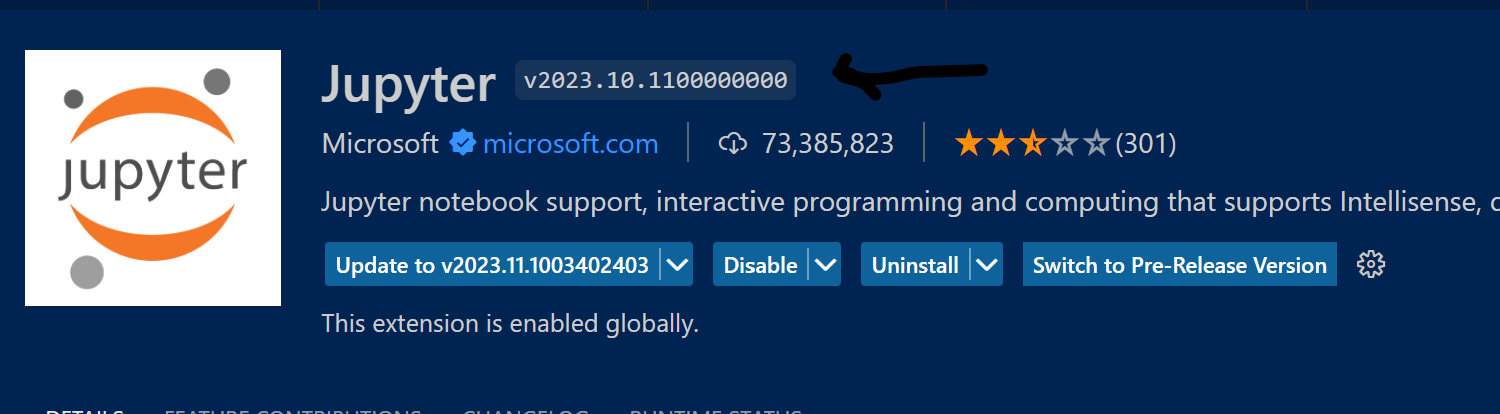
\includegraphics[scale = 0.3]{attachment/chapter_AML/Scc018}
	\caption{Rollback version}
\end{figure}

\subsubsection{Tunnel Connection}
With the option to connect to the workspace it self, the blobstorage, where the notebooks of each user are stored, can be access. To to this \gls{vsc} connected via tunnel to the workspace with the compute instance in the web browser or with the desktop application.
 
\begin{figure}[H]
	\centering
	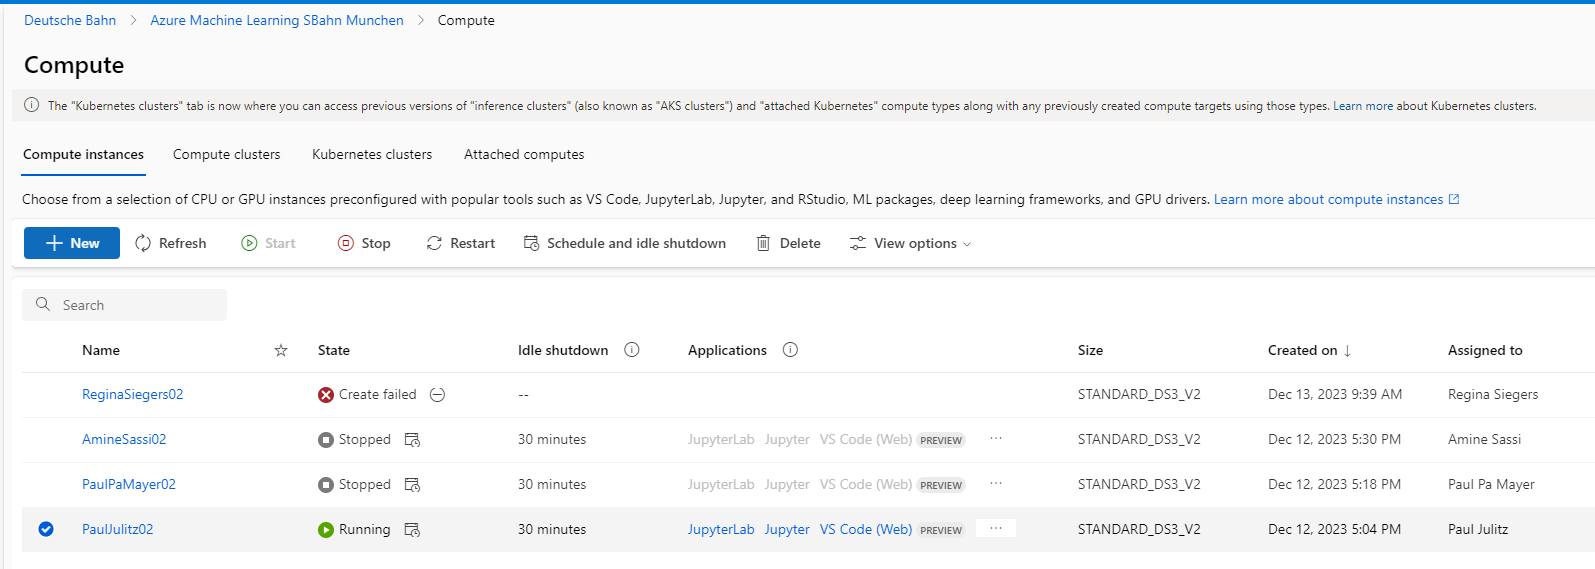
\includegraphics[scale = 0.3]{attachment/chapter_AML/Scc022}
	\caption{Create a tunnel connection}
\end{figure}

On the bottom left (1) the tunnel connection is displayed. The internal file system gets linked as the storage (2), where the notebook can be access. Note: Locally stored notebooks can be used by the previous section.

\begin{figure}[H]
	\centering
	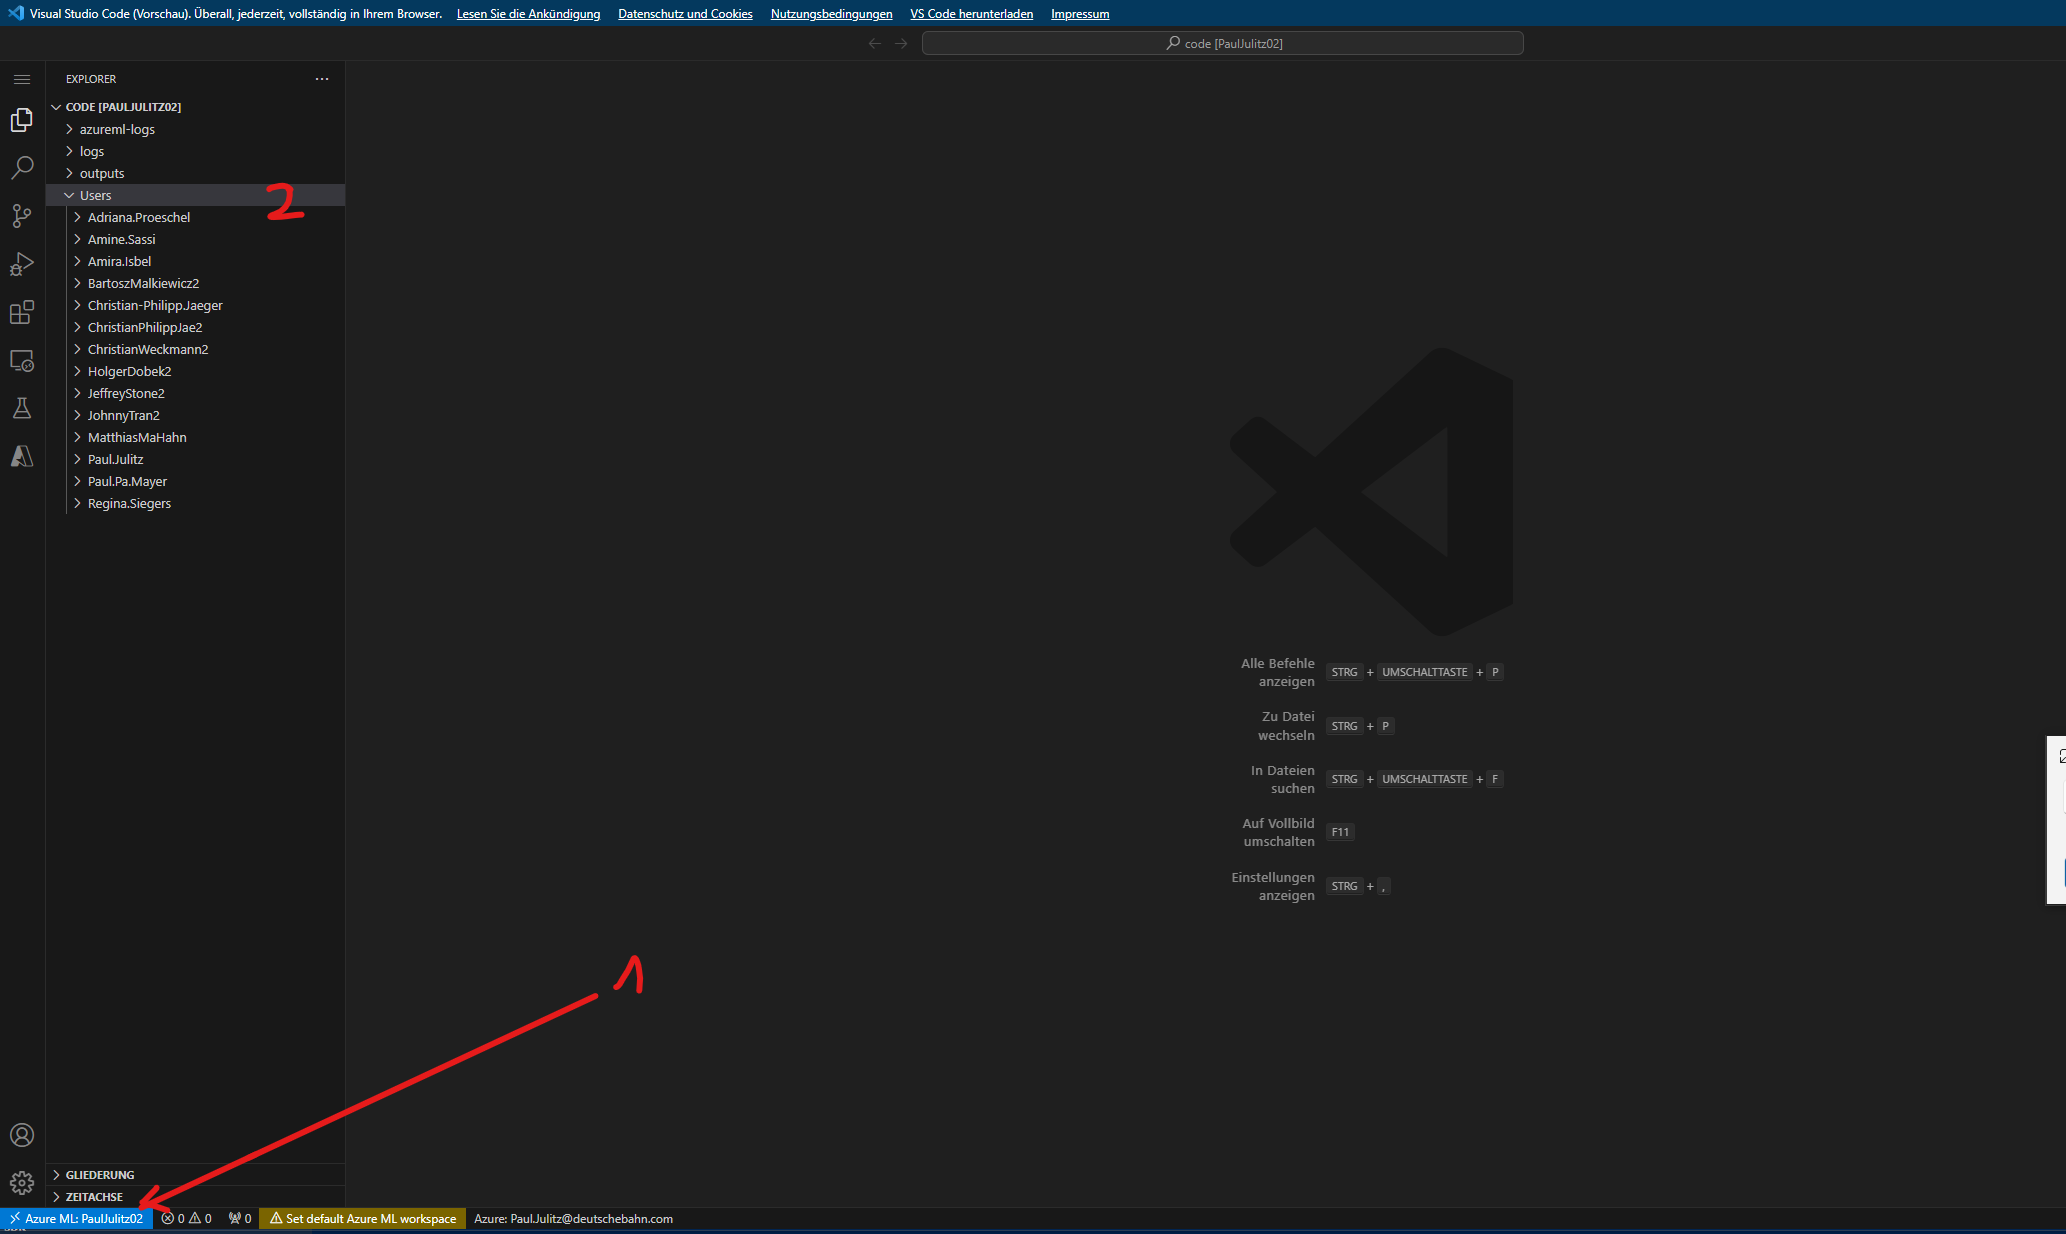
\includegraphics[scale = 0.2]{attachment/chapter_AML/Scc021}
	\caption{Create a tunnel connection}
\end{figure}

\subsubsection{Handle to Worksapce using SDK v2}

With the parameters that identify the workspace, we will use the \textit{MLClient} from \gls{AMLSDKv2} (\textit{azure.ai.ml}) to handelt the workspace. The default authentication is \textit{DefaultAzureCredentail()}.There are more ways to to configure the credential, see \href{https://docs.microsoft.com/en-us/python/api/azure-identity/azure.identity.defaultazurecredential?view=azure-python}{default azure authentication}.\\


The first setup, it to connect to the worksppace and retriev metainformation about the worksapce it self.
\begin{lstlisting}[language=iPython]
# import required libraries
from azure.ai.ml import MLClient
from azure.ai.ml import command, Input
from azure.identity import DefaultAzureCredential
# system libraries
import os

# Using local configuration (.env)
subscription_id = os.environ["SUBSCRIPTION_ID"]
resource_group = os.environ["RESOURCE_GROUP"]
workspace = os.environ["WORKSPACE_NAME"]

# get a handle to the workspace
ml_client = MLClient(
DefaultAzureCredential(), subscription_id, resource_group, workspace
)

for ws in ml_client.workspaces.list():
print(ws.name, ":", ws.location, ":", ws.description)
\end{lstlisting}

\paragraph{Problem Retrieve a token}
In the first approach to connect to the workspace via vscode an authentication problem accures
\begin{lstlisting}[style=CMD]
	DefaultAzureCredential failed to retrieve a token from the included credentials.
	Attempted credentials:
	EnvironmentCredential: EnvironmentCredential authentication unavailable. Environment variables are not fully configured.
	Visit https://aka.ms/azsdk/python/identity/environmentcredential/troubleshoot to troubleshoot.this issue.
	ManagedIdentityCredential: ManagedIdentityCredential authentication unavailable, no response from the IMDS endpoint.
	SharedTokenCacheCredential: Azure Active Directory error '(invalid_grant) AADSTS700082: The refresh token has expired due to inactivity. The token was issued on 2023-10-10T08:52:54.9825803Z and was inactive for 90.00:00:00. Trace ID: 1170c2c8-e350-4293-a848-6d9677a51c00 Correlation ID: 8092aa76-93b3-4150-b342-afdba943c2c3 Timestamp: 2024-01-13 17:38:27Z'
	Content: {"error":"invalid_grant","error_description":"AADSTS700082: The refresh token has expired due to inactivity. The token was issued on 2023-10-10T08:52:54.9825803Z and was inactive for 90.00:00:00. Trace ID: 1170c2c8-e350-4293-a848-6d9677a51c00 Correlation ID: 8092aa76-93b3-4150-b342-afdba943c2c3 Timestamp: 2024-01-13 17:38:27Z","error_codes":[700082],"timestamp":"2024-01-13 17:38:27Z","trace_id":"1170c2c8-e350-4293-a848-6d9677a51c00","correlation_id":"8092aa76-93b3-4150-b342-afdba943c2c3","error_uri":"https://login.microsoftonline.com/error?code=700082"}
	To mitigate this issue, please refer to the troubleshooting guidelines here at https://aka.ms/azsdk/python/identity/defaultazurecredential/troubleshoot.
\end{lstlisting}

The \href{https://github.com/Azure/azure-sdk-for-python/blob/main/sdk/identity/azure-identity/TROUBLESHOOTING.md#troubleshoot-environmentcredential-authentication-issues}{the troubleshot for authentication issues} didn't result in any solution for the problem.\\

The fix was to use \verb+DefaultAzureCredential(exclude_shared_token_cache_credential=True)+. The hypothesis it that it resets the retrieved token, and therefore resolved the token problem, see \href{https://github.com/Azure/azure-sdk-for-python/issues/29040}{Solution}


\subsection{MLflow}

\mlflow is a open source framework for managing the \gls{ML} life cycle. It allows a consistent set of tools regardless of where the experiment is running locally, a \gls{VM} or on an \Azure compute instance. The \gls{AML} is compatatible with mlflow.

In the example \textit{diabetes single steps} the model used mlflow for tracking relevant information for the experiments.
\begin{lstlisting}[language=iPython]
	import src.main as main
	
	# parse arguments
	args = main.parse_args()
	
	# run main function/ return model
	model = main.main(args)
\end{lstlisting}
The output of mlflow returned:
\begin{lstlisting}[style=CMD]
	2024/01/20 11:05:21 INFO mlflow.tracking.fluent: Autologging successfully enabled for sklearn.
	2024/01/20 11:05:21 INFO mlflow.utils.autologging_utils: Created MLflow autologging run with ID '3ecc9f78851941a39a8cf977f6d137df', which will track hyperparameters, performance metrics, model artifacts, and lineage information for the current sklearn workflow
\end{lstlisting}
\textit{Note:} To return the model is not necessarly required. was not required.
To open the mlflow web interface, you enter 
\begin{lstlisting}[style=CMD]
	mlflow ui
\end{lstlisting}
This will return the ip adress
\begin{lstlisting}[style=CMD]
	INFO:waitress:Serving on http://127.0.0.1:5000	
\end{lstlisting}
Until the mlflow service is available, the execution is still running, therefore the execution of the command is not complete. To exit, press \verb+CTL and C+ or \verb+str and C+.
\begin{lstlisting}[style=CMD]
	(Icarus_v4) PS C:\Users\PaulJulitz\Documents\GitHub\Emmy_ML_One> mlflow ui                    
	INFO:waitress:Serving on http://127.0.0.1:5000
	# Press str + c
	Aborted!
\end{lstlisting}



\begin{figure}[H]
	\centering
	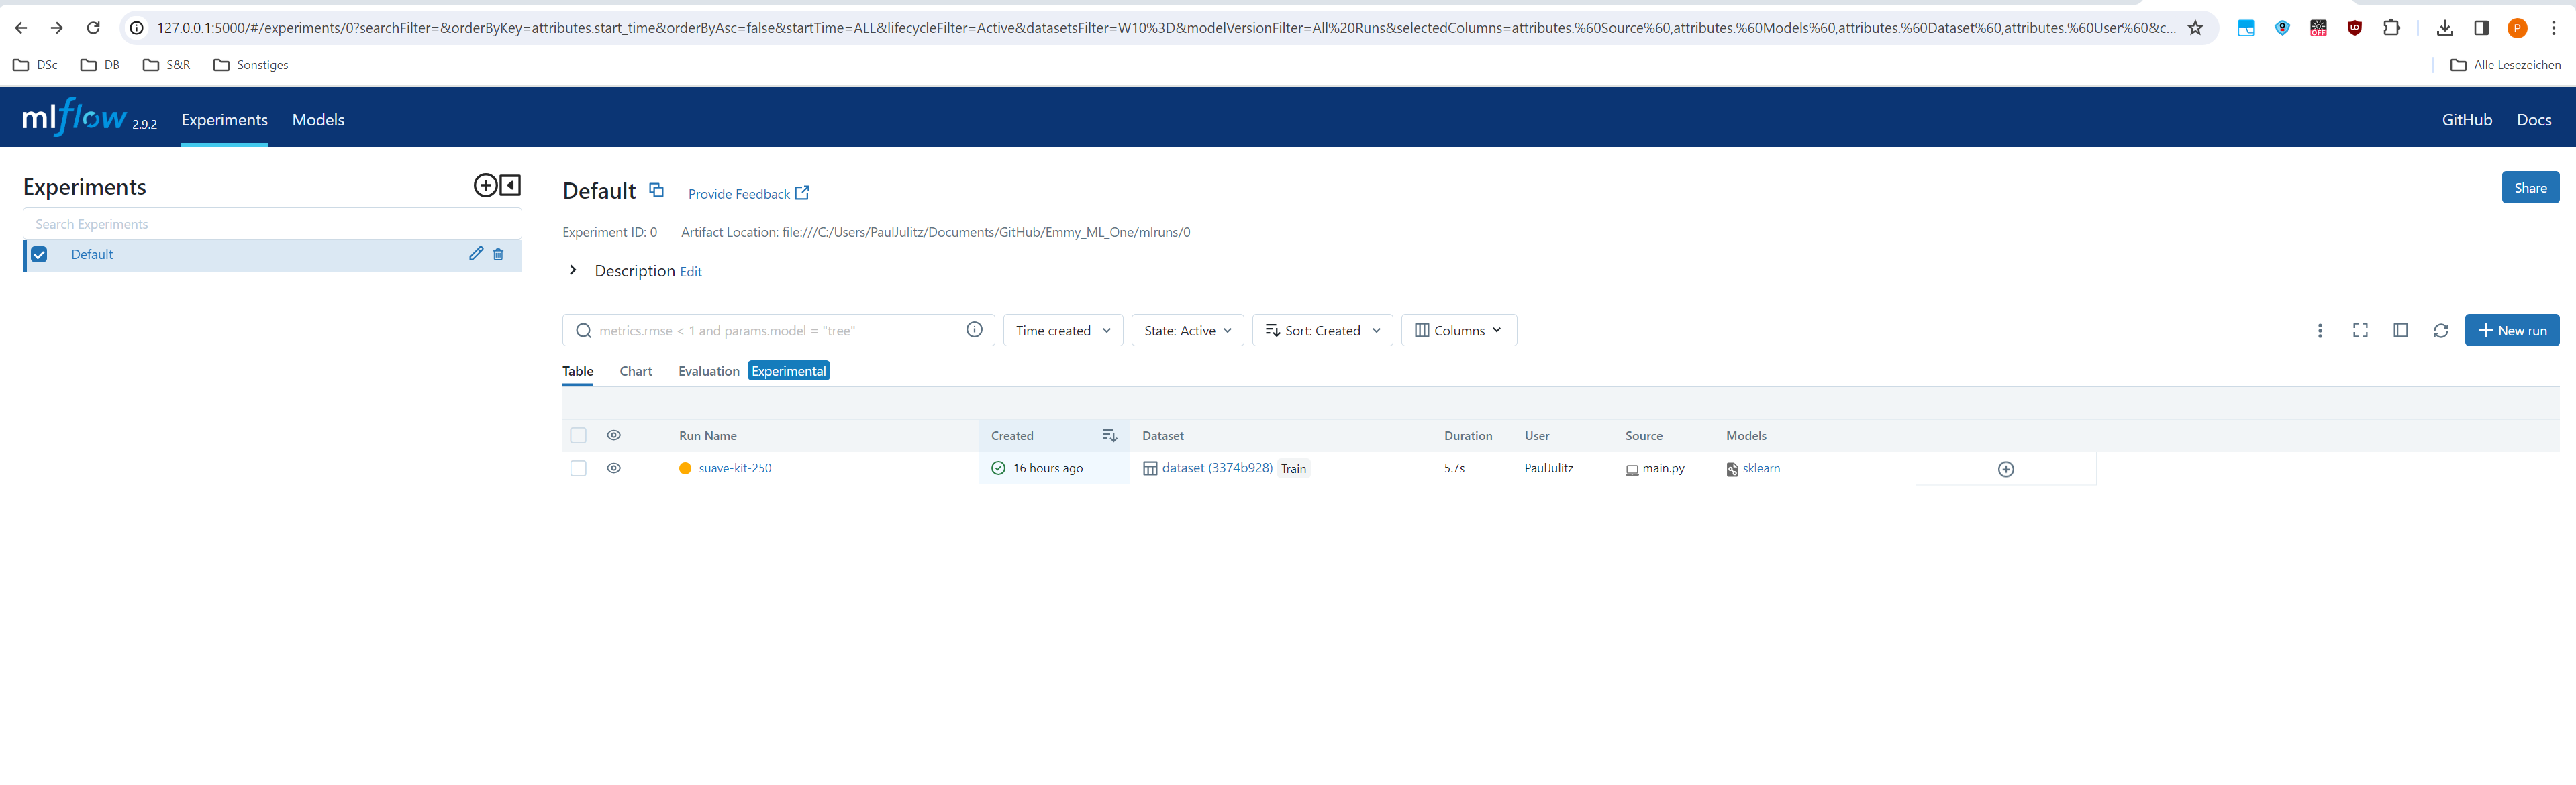
\includegraphics[scale = 0.2]{attachment/chapter_AML/Scc029}
	\caption{Open Web Interface}
	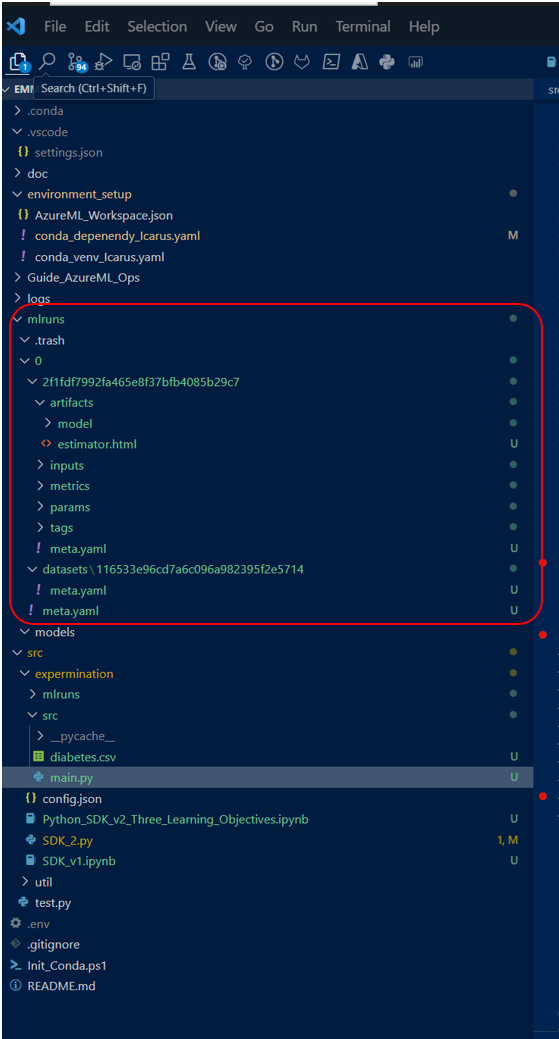
\includegraphics[scale = 0.4]{attachment/chapter_AML/Scc031}
	\caption{Execution local, therefore mflow stored local}
\end{figure}

The web interface allows to see information about the model artefact, metrics, used parameters, schema information about the data used for the training.

\begin{figure}[H]
	\centering
	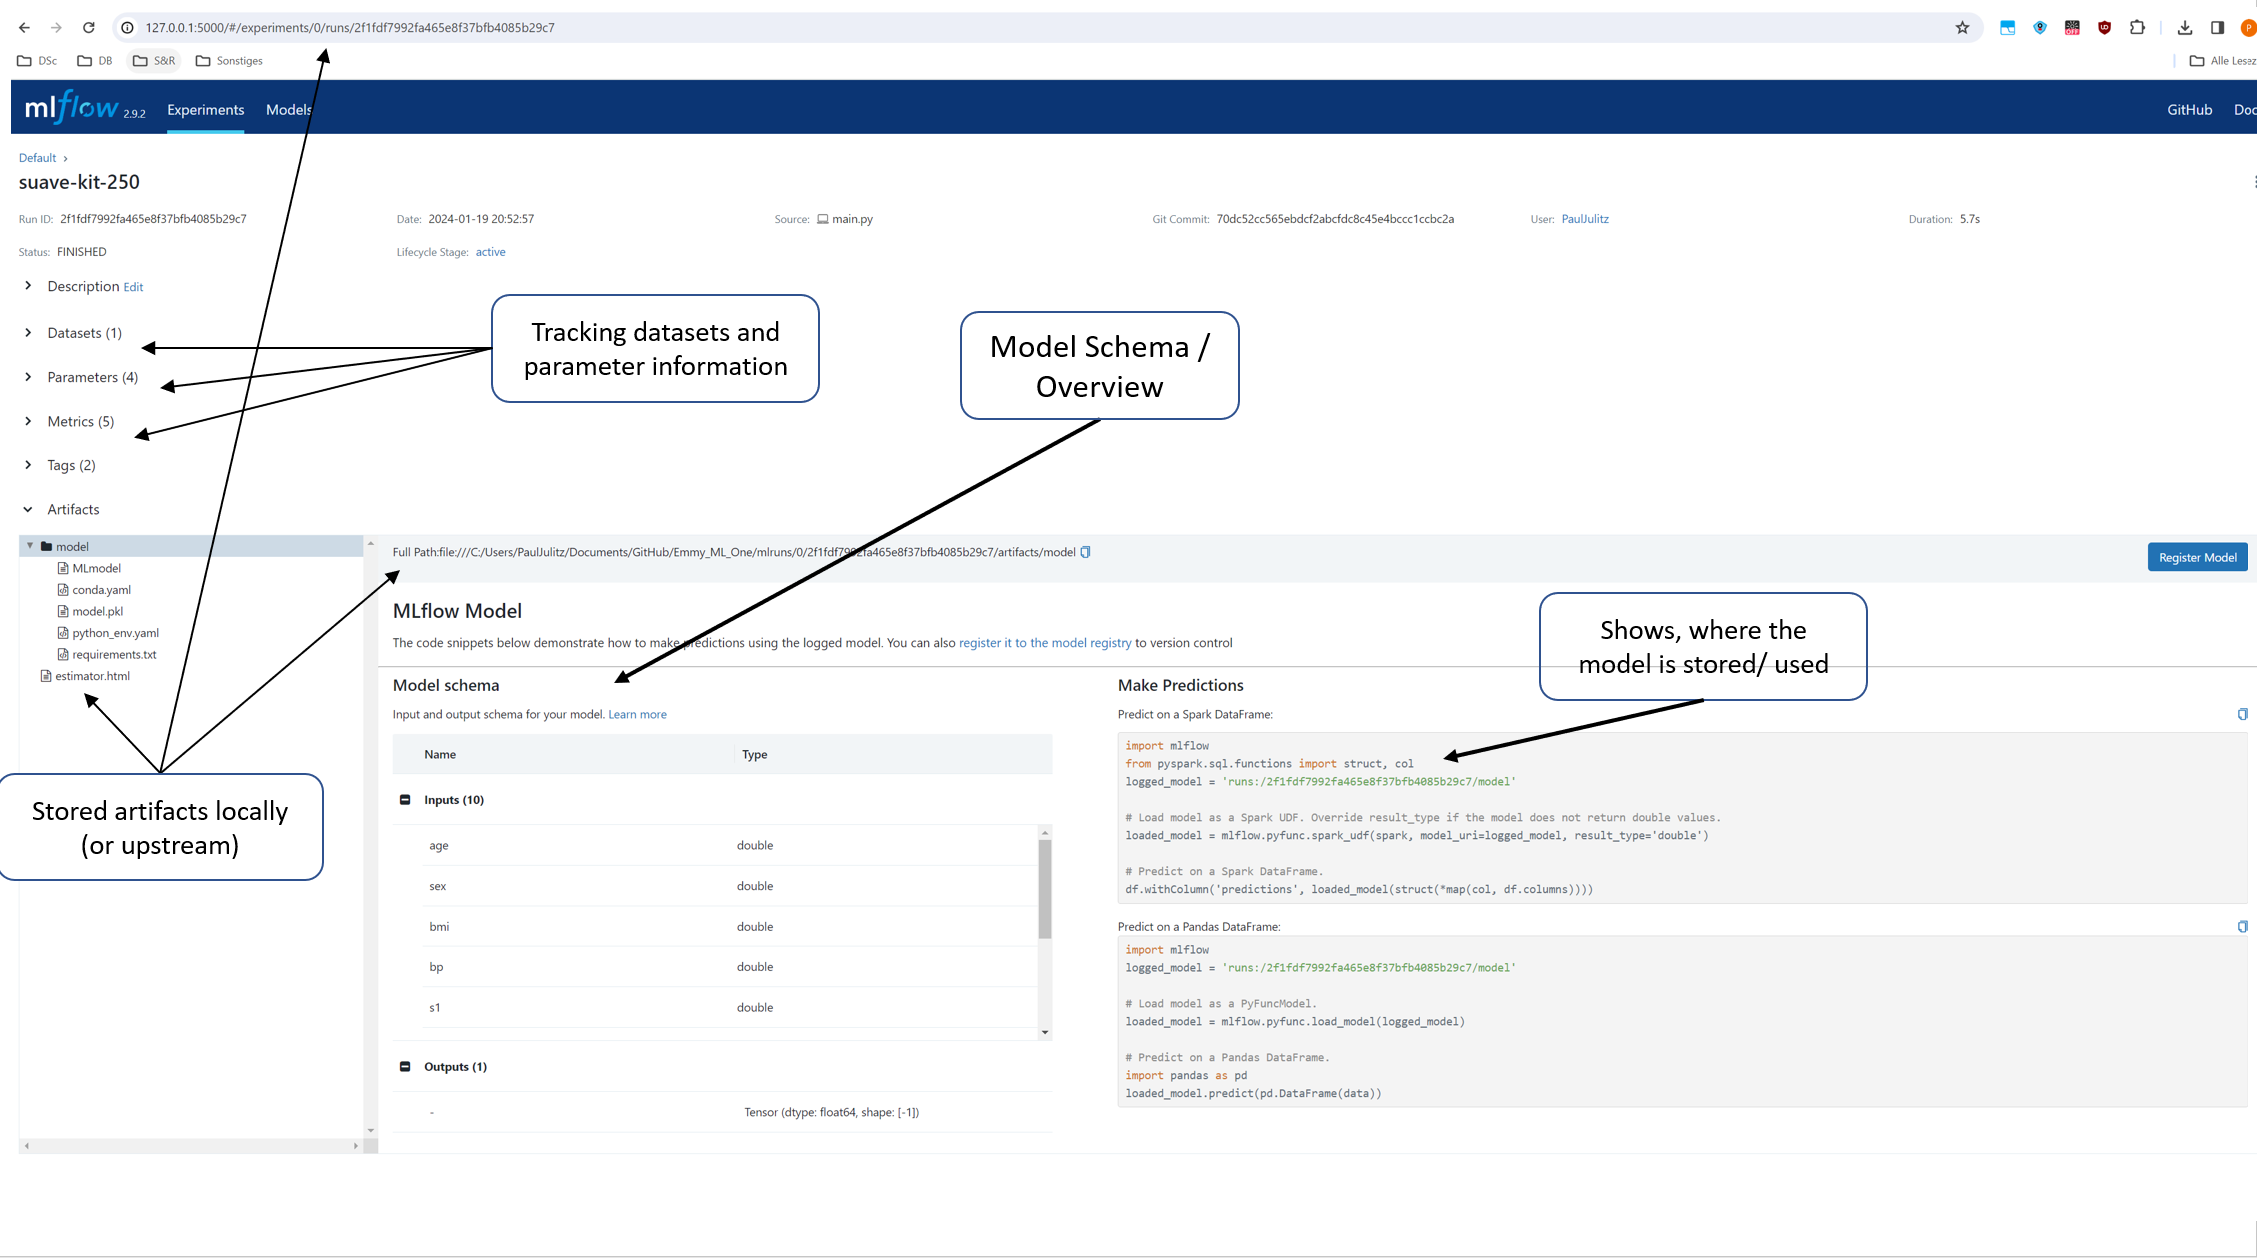
\includegraphics[scale = 0.4]{attachment/chapter_AML/Scc030}
	\caption{Overview mlflow local server}
\end{figure}

Note: To use the model, it first has to be registered, see the information after \textit{MLflow Model}.
\begin{lstlisting}[language=iPython]
	#...
	# Log the sklearn model and register as version 1
	mlflow.sklearn.log_model(
	sk_model=model,
	artifact_path="sklearn-model",
	signature=signature,
	registered_model_name="sk-learn-random-forest-reg-model",
	)
\end{lstlisting}
To update the model, you can use 
%\href{https://www.mlflow.org/docs/latest/model-registry.html#adding-an-mlflow-model-to-the-model-registry}{adding model (mlflow)
	\begin{lstlisting}[language=iPython, caption={See comment},captionpos=b]
		result = mlflow.register_model(
		"runs:/d16076a3ec534311817565e6527539c0/sklearn-model", "sk-learn-random-forest-reg"
		)
	\end{lstlisting}
	For reference the url is stored her as a comment.
	

\subsection{Command a Job}
To command a job, two parts are made. The first one, is to configure the job command the secound is to create a script, which handels the dataprocessing, splitting and train data based on a given model, and then returns a output model. In the example, the first part looks like this:

\begin{lstlisting}[language=iPython, caption={Example command configuration},captionpos=b]
	# create the command
	job = command(
	code="./src",  # local path where the code is stored
	command="python main.py --diabetes-csv ${{inputs.diabetes}}",
	inputs={
		"diabetes": Input(
		type="uri_file",
		path="https://azuremlexamples.blob.core.windows.net/datasets/diabetes.csv",
		)
	},
	environment="AzureML-sklearn-1.0-ubuntu20.04-py38-cpu@latest",
	display_name="sklearn-diabetes-example",
	# description,
	# experiment_name
	)
\end{lstlisting}

\paragraph{Building the python command}
The \verb+job = command(..)+ allows for a variate of configuration. In this example the \textit{command} is configured like:

\begin{center}\verb+python main.py --diabetes-csv ${{inputs.diabetes}}+.\end{center}

\begin{description}
	\item[Double Hyphen] The $- -$ are a \gls{CMD} standard to indicate \text{options} or \text{flags}. The function \verb+main()+ can reseve the argument \verb+diabetes-csv+. This standard separate \textit{command-line option} from the actually value it self.
	\item[Dollar Sign] The $\$$ are indicate that the following expression gets evaluated. It is a marker to evaluate the following variable expression. In conjunction with the hyphen $--$ allows to define the value of a command expression at the moment of running instead of specifying it in the code itself. 
	\begin{lstlisting}[style=CMD]
	(Icarus_v4) PS C:\Users\PaulJulitz\Documents\GitHub\Emmy_ML_One> Write-Output $("hello")
	hello
	\end{lstlisting}
	\item[Double Curly Bracktes] The $\left\lbrace \left\lbrace \dots \right\rbrace\right\rbrace$ are used as variable interpolation in configuration. In this example the \verb+command()+ takes in as an dictionary the argument \verb+input+. The expression \verb+$ {{input.diabetes}}+ returns the \textit{url path}. My assumption is, that inside the \verb+command()+ the returned dictionary from \verb+input()+, get the file path extracted, if the entries are valied, see Literal types under \ref{subsec:azure-ai-ml-Input}. Note: As a normal dictionary read, my read would be, that \verb+input.diabetes+ would return a dictionary and not the file path.
\end{description} 

The command can therefore be read as $"$\verb+python main. py --diabetes-csv=https://azuremlexamples.blob.core.windows.net/datasets/diabetes.csv+. Inside the main.py \verb+--diabetes-csv+ is then used as followed
\begin{lstlisting}[language=iPython]
	df = pd.read_csv(filepath_or_buffer="https://azuremlexamples.blob.core.windows.net/datasets/diabetes.csv")
\end{lstlisting}

\paragraph{Pasing argumentes for the main() function: *args, *kargs, argparse}
\href{https://docs.python.org/3/library/argparse.html}{Referenz argpase}

The \verb+main.py+ uses the \verb+argparse+ library. It is a parser for command-line option, arguments. That means parsed arguments from the command-line are \textbf{first run through} the \verb+argpase.AddArgumentParser()+ before it parsed as arguments for the \verb+main()+ function. 
\begin{lstlisting}[language=iPython]
def parse_args():
# setup arg parser
parser = argparse.ArgumentParser()

# add arguments
parser.add_argument("--diabetes-csv", type=str)
parser.add_argument("--random_state", type=int, default=42)
parser.add_argument("--fit_intercept", type=bool, default=True)
parser.add_argument("--positive", type=bool, default=False)

# parse args
args = parser.parse_args()

# return args
return args

# run script
if __name__ == "__main__":
# parse args
args = parse_args()

# run main function
main(args)
\end{lstlisting}

Then the parsed arguments are used by the \verb+main()+ function as
\begin{lstlisting}[language=iPython]
def main(args): # <---- args as input are specified
# enable auto logging
mlflow.autolog()

# read in data
df = pd.read_csv(args.diabetes_csv) # <---- FIRST USE

# process data
X_train, X_test, y_train, y_test = process_data(df, args.random_state) # <---- SECOND USE

# setup parameters
params = {
	"fit_intercept": args.fit_intercept, # <---- THIRD USE
	"positive": args.positive, # <---- FORTH USE
}    

# train model
train_model(params, X_train, X_test, y_train, y_test)
\end{lstlisting}

\paragraph{Possible output}
If the main function returns the trained model, then the output looks like
\begin{lstlisting}[language=iPython]
	# main()
	#...
	# train model
	return train_model(params, X_train, X_test, y_train, y_test)
	
	# main.py
	ic(main(args))
\end{lstlisting}
\begin{lstlisting}[style=CMD, caption={Output of the ic() function, captionpos=b}]
array([  37.90031426, -241.96624835,  542.42575342,  347.70830529,
-931.46126093,  518.04405547,  163.40353476,  275.31003837,
736.18909839,   48.67112488])
\end{lstlisting}



